% ============================================================
%  main.tex  —  A Regime-Switching Framework for Tactical Sector Tilts
%  Preslav Vachev, emlyon business school, May 2026
% ============================================================
\documentclass[11pt, a4paper]{article}

% ── Packages ────────────────────────────────────────────────
\usepackage[T1]{fontenc}
\usepackage[utf8]{inputenc}
\usepackage{mathptmx}           % Times New Roman body + math
%% PAGE BUDGET: competition limit is 5--7 pages EXCLUDING appendices.
%% Body was 16 pages at 12pt/onehalfspacing/3cm margins. Compacted here.
%% If still over, next levers in order: 10pt -> \setstretch{1.0} -> margins 2.0cm.
\usepackage[
  top=1.6cm, bottom=1.6cm,
  left=1.6cm, right=1.6cm
]{geometry}
\usepackage{setspace}
\usepackage{amsmath, amssymb}
\usepackage{graphicx}
\usepackage{booktabs}
\usepackage{multirow}
\usepackage{array}
\usepackage{longtable}
\usepackage{pdflscape}
\usepackage{rotating}          % sidewaysfigure: rotates figure + caption together
\usepackage{tabularx}
\usepackage{xcolor}
%% \new{} is a no-op: change-tracking is switched off. Red is now reserved for
%% \textcolor{red}{[PV: ...]} items that still need a decision.
\newcommand{\new}[1]{#1}
\usepackage{soul}               % \hl{} highlighting
\usepackage{tcolorbox}          % fact-check boxes (pulls in tikz/pgf, but NOT its libraries)
\usepackage{tikz}               % explicit, so the dependency is not accidental
\usetikzlibrary{positioning, arrows.meta}   % required by figures/fig_pipeline.tex
\usepackage[hang, flushmargin]{footmisc}
\usepackage{caption}
\usepackage{float}
\usepackage{enumitem}
\usepackage{verbatim}
\usepackage{placeins}
\usepackage{fancyhdr}           % \FloatBarrier
\usepackage{titlesec}
\usepackage{parskip}
% bibliography handled manually in References section
\definecolor{elsblue}{RGB}{0,84,166}   % Elsevier-style link/citation blue
%% \cit{key}{text} -> blue in-text citation hyperlinked to its reference entry.
%% Each entry in the reference list carries a matching \reftgt{key}.
\newcommand{\cit}[2]{\hyperlink{ref:#1}{\textcolor{elsblue}{#2}}}
\newcommand{\reftgt}[1]{\hypertarget{ref:#1}{}}
\usepackage[
  colorlinks=true,
  linkcolor=elsblue,
  citecolor=elsblue,
  urlcolor=elsblue
]{hyperref}

% ── Typography ───────────────────────────────────────────────
\setstretch{1.05}
\setlength{\parindent}{0pt}
\setlength{\parskip}{3pt}

% ── Section formatting ───────────────────────────────────────
\titleformat{\section}{\large\bfseries}{\thesection.}{0.5em}{}
\titleformat{\subsection}{\normalsize\bfseries}{\thesubsection}{0.5em}{}
\titlespacing*{\section}{0pt}{9pt}{3pt}
\titlespacing*{\subsection}{0pt}{6pt}{2pt}

% ── Fact-check box ───────────────────────────────────────────
\newtcolorbox{factcheck}{
  colback=yellow!20, colframe=red!60!black,
  fonttitle=\bfseries\small, title={\textcolor{red!70!black}{FACT-CHECK REQUIRED}},
  left=4pt, right=4pt, top=4pt, bottom=4pt, boxrule=0.8pt
}

% ── Figure/table placeholder ─────────────────────────────────
\newtcolorbox{placeholder}[1]{
  colback=blue!5, colframe=blue!40,
  fonttitle=\bfseries\small\color{blue!60!black},
  title={#1}, left=4pt, right=4pt, top=4pt, bottom=4pt,
  boxrule=0.6pt
}

% ── Float packing ────────────────────────────────────────────
%% LaTeX defaults refuse to place a large float on a page that also carries
%% text, which left whole pages two-thirds blank. These let floats share pages.
\renewcommand{\topfraction}{0.92}
\renewcommand{\bottomfraction}{0.85}
\renewcommand{\textfraction}{0.06}
\renewcommand{\floatpagefraction}{0.85}
\setcounter{topnumber}{3}
\setcounter{bottomnumber}{2}
\setcounter{totalnumber}{4}

% ── Caption style ────────────────────────────────────────────
\captionsetup{font=small, labelfont=bf, skip=4pt}

% ── Bibliography file ────────────────────────────────────────


% ============================================================
%% ANONYMITY SWITCH -- declared in the preamble so the running footer can use it.
%% Competition rules: "The cover page should contain only the title but not the
%% candidate or university name"; reports are judged anonymously.
%%   \anonymoustrue  -> title only, no name in footer  (USE FOR THE CFA SUBMISSION)
%%   \anonymousfalse -> named cover + footer           (use for supervisor drafts)
\newif\ifanonymous
\anonymousfalse

\begin{document}

% ── Footer ─────────────────────────────────────────────────────────────
\pagestyle{fancy}
\fancyhf{}
\renewcommand{\headrulewidth}{0pt}
\ifanonymous\else\fancyfoot[C]{\small Vachev, P.}\fi
\fancyfoot[R]{\small \thepage}
\fancypagestyle{plain}{%
  \fancyhf{}%
  \renewcommand{\headrulewidth}{0pt}%
  \ifanonymous\else\fancyfoot[C]{\small Vachev, P.}\fi
  \fancyfoot[R]{\small \thepage}%
}


% ── Title page ──────────────────────────────────────────────
\begin{titlepage}
  \thispagestyle{empty}
  \centering
  \ifanonymous
    \vspace*{\fill}
    {\LARGE\bfseries A Regime-Switching Framework for Tactical Sector Tilts\\[0.4em]
     under Higher-Moment Investor Preferences}
    \vspace*{\fill}
  \else
    \vspace*{2cm}
    {\small Vachev, P.\ --- Dissertation --- May 2026}\\[0.3cm]
    {\LARGE\bfseries A Regime-Switching Framework for Tactical Sector Tilts\\[0.4em]
     under Higher-Moment Investor Preferences}\\[2cm]
    {\large\itshape Preslav Vachev}\\[0.5cm]
    {\normalsize emlyon business school}\\[1.5cm]
    {\normalsize Supervisor: Professor Bertrand Tavin \quad|\quad May 2026}
  \fi
  \vfill
\end{titlepage}
\pagenumbering{arabic}

\clearpage

% ── Abstract ────────────────────────────────────────────────
\begin{abstract}
\noindent
This paper develops and evaluates a regime-aware core-plus-satellite allocation framework
designed for implementation within the operational constraints of a wealth management context.
A three-state Hidden Markov Model is estimated on monthly excess log returns of the S\&P~500
Total Return index and the Bloomberg US Treasury 7--10 Year index. The resulting one-step-ahead
predictive regime probabilities serve as the signal for a scoring engine that evaluates nine US
sector ETFs and gold as candidate tilts against a 60/40 benchmark. Tilt scoring follows a
Taylor-expanded expected utility function \cit{jondeau2006}{(Jondeau and Rockinger 2006)}, accommodating
mean-variance, mean-variance-skewness, and mean-variance-kurtosis investor types, and a rolling
60-month estimation window allows the model to adapt to structural breaks in sector leadership.
\new{A score improvement floor holds the portfolio in the passive core in any month in which no
candidate tilt improves on it by more than the floor. Three further mechanisms target drawdown
protection, none of which lets the volatility or correlation signals reach selection: a
style-dependent displacement rule funds cyclical tilts pro-rata from the whole core and
defensive tilts from the equity leg alone, so the bond block stays intact in risk-off months. A
downside realised-semivariance ratio computed from daily returns sharpens the bear probability
that sizes the satellite sleeve, and a blended bond--equity correlation sets the internal
equity--bond split of the core. At a 30\% satellite sleeve the framework
achieves a CAGR of 9.26\% against a benchmark of 7.74\%, a Sharpe ratio of 1.029 versus 0.874,
a maximum drawdown of $-26.6$\% versus $-30.6$\%, and a downside deviation of 6.99\% versus
7.07\%, improving on the benchmark on every risk-adjusted metric simultaneously. A 35\%
sleeve raises CAGR to 9.64\% at a Sharpe ratio of 1.039. At both operating points up-capture
exceeds 102\% of the benchmark while down-capture remains below 90\%.}
\end{abstract}

\vspace{6pt}
\noindent\textbf{Keywords:} Portfolio optimization, tactical asset allocation, market regimes, sector rotation, higher-moment preferences

\vspace{4pt}
\noindent\textbf{JEL Classification:} G11 $\cdot$ G17 $\cdot$ C22

\section{Introduction}
% ============================================================

In the wealth management business, only a small percentage of clients are managed actively, and
that depends largely on the size and the cost of continuing operations of the firm. Most
individual clients are managed passively or on very infrequent rebalancing schedules, and their
portfolios are standardised to facilitate the communication chain between client, relationship
manager, portfolio manager, and trading desk, and to abide by rules and regulations. The
operational economics are the reason. \cit{pwc2025}{(PwC 2025)} projects passive assets to reach USD~70 trillion by
2030, while 89\% of asset managers report profitability pressure and profit per unit of AUM has
declined by roughly 19\% since 2018. Under that combination of cost pressure and growing
assets, a standardised passive mandate is the practical default for smaller clients, which
makes improving what it delivers worth as much to the firm as to the client.

This poses the question at the core of this study: is it possible to develop a model with a
decision tilt that outperforms a passive benchmark on a risk-adjusted basis and that
simultaneously addresses the concerns of investors with different preferences for higher moments?
Most studies that use a regime switching framework to solve a portfolio allocation problem do so
considering different types of investors, but not the type of portfolio manager who operates
within a standardised, constrained mandate. This study deliberately caters to both audiences.

Headline performance is reported in Section~\ref{sec:results}, with the full sensitivity grid across sleeve sizes and investor types in Appendix~\ref{sec:appendix_all}. We contribute
to the regime-switching and portfolio allocation literature in four ways. First, the HMM is
refit at every rebalance date within a rolling 60-month window, allowing the model to adapt to
structural breaks in sector leadership. Second, allocation decisions are made based on a 
scoring mechanism. Third, multiple investor preference types, from mean-variance to 
mean-variance-kurtosis, are accommodated within the same framework. Finally, a score improvement 
floor acts as a hurdle rate, so the model deviates from the passive core only when the 
regime signal justifies it.

\new{These four elements define the selection engine, which scores candidate tilts on the
predictive moments of the regime mixture alone. We extend that engine with three mechanisms
aimed at drawdown protection: a style-dependent displacement
rule that funds cyclical tilts pro-rata from the core and defensive tilts from equity alone, so
the bond block survives risk-off months. A downside realised-semivariance signal from daily
returns sharpens the bear probability sizing the sleeve, and a blended bond--equity correlation
sets the internal equity--bond split of the core. Selection is insulated from the volatility and correlation signals, which act only at
the sizing stage. The displacement rule is applied identically to every candidate, so it shapes
how a tilt is funded without influencing which tilt is chosen. That separation means the same
mechanism can be used outside this setting, wherever an exposure needs to be scaled by the
estimated regime probabilities.}

\section{Data}
\label{sec:data}
% ============================================================

In order to define the regimes, one broad equity index and one broad bond index were used:
the S\&P~500 total return index and the Bloomberg US Treasury 7--10 Year index (LT09TRUU).
These monthly returns were continuously compounded. The S\&P~500 total return series was
obtained through the Yahoo Finance API as a daily dataset, and the Bloomberg Treasury index 
through Bloomberg. Because a daily history of LT09TRUU was not available to us, 
the iShares 7--10 Year Treasury Bond ETF (IEF) is used as a signal-side proxy for the bond leg
The 1-month T-Bill rate was subtracted from both to calculate the excess log return, which is
how both series are referred to in this study. The monthly T-Bill simple return was acquired
through the official Fama-French website and converted to log return for comparability with
the other data. The start of the sample period for constructing the HMM is January 1999 and
the end date is July 2026, matched to the issuance dates of the sector ETFs used for
satellite tilts.

For the satellite universe, this study uses the nine State Street SPDR sector ETFs: Materials
(XLB), Energy (XLE), Financials (XLF), Industrials (XLI), Technology (XLK), Consumer
Staples (XLP), Utilities (XLU), Health Care (XLV), and Consumer Discretionary (XLY). Gold
(XAU) is included as a tenth satellite candidate. All nine sector ETF return series were obtained through the Yahoo Finance API. The gold (XAU) return series was obtained from Bloomberg. Descriptive statistics and the pairwise correlation matrix are reported in Tables~\ref{tab:data_stats} and~\ref{tab:correlations}.

\textbf{Figure~\ref{fig:price_levels}} shows the full price history of all twelve assets. Together, the S\&P~500 TR and LT09TRUU constitute the 60/40 benchmark core at a
fixed weight allocation. The choice of a 60/40 split is the industry standard for a balanced
client mandate and represents the passive baseline against which all strategy configurations
are evaluated.

\begin{figure}[t]
  \centering
  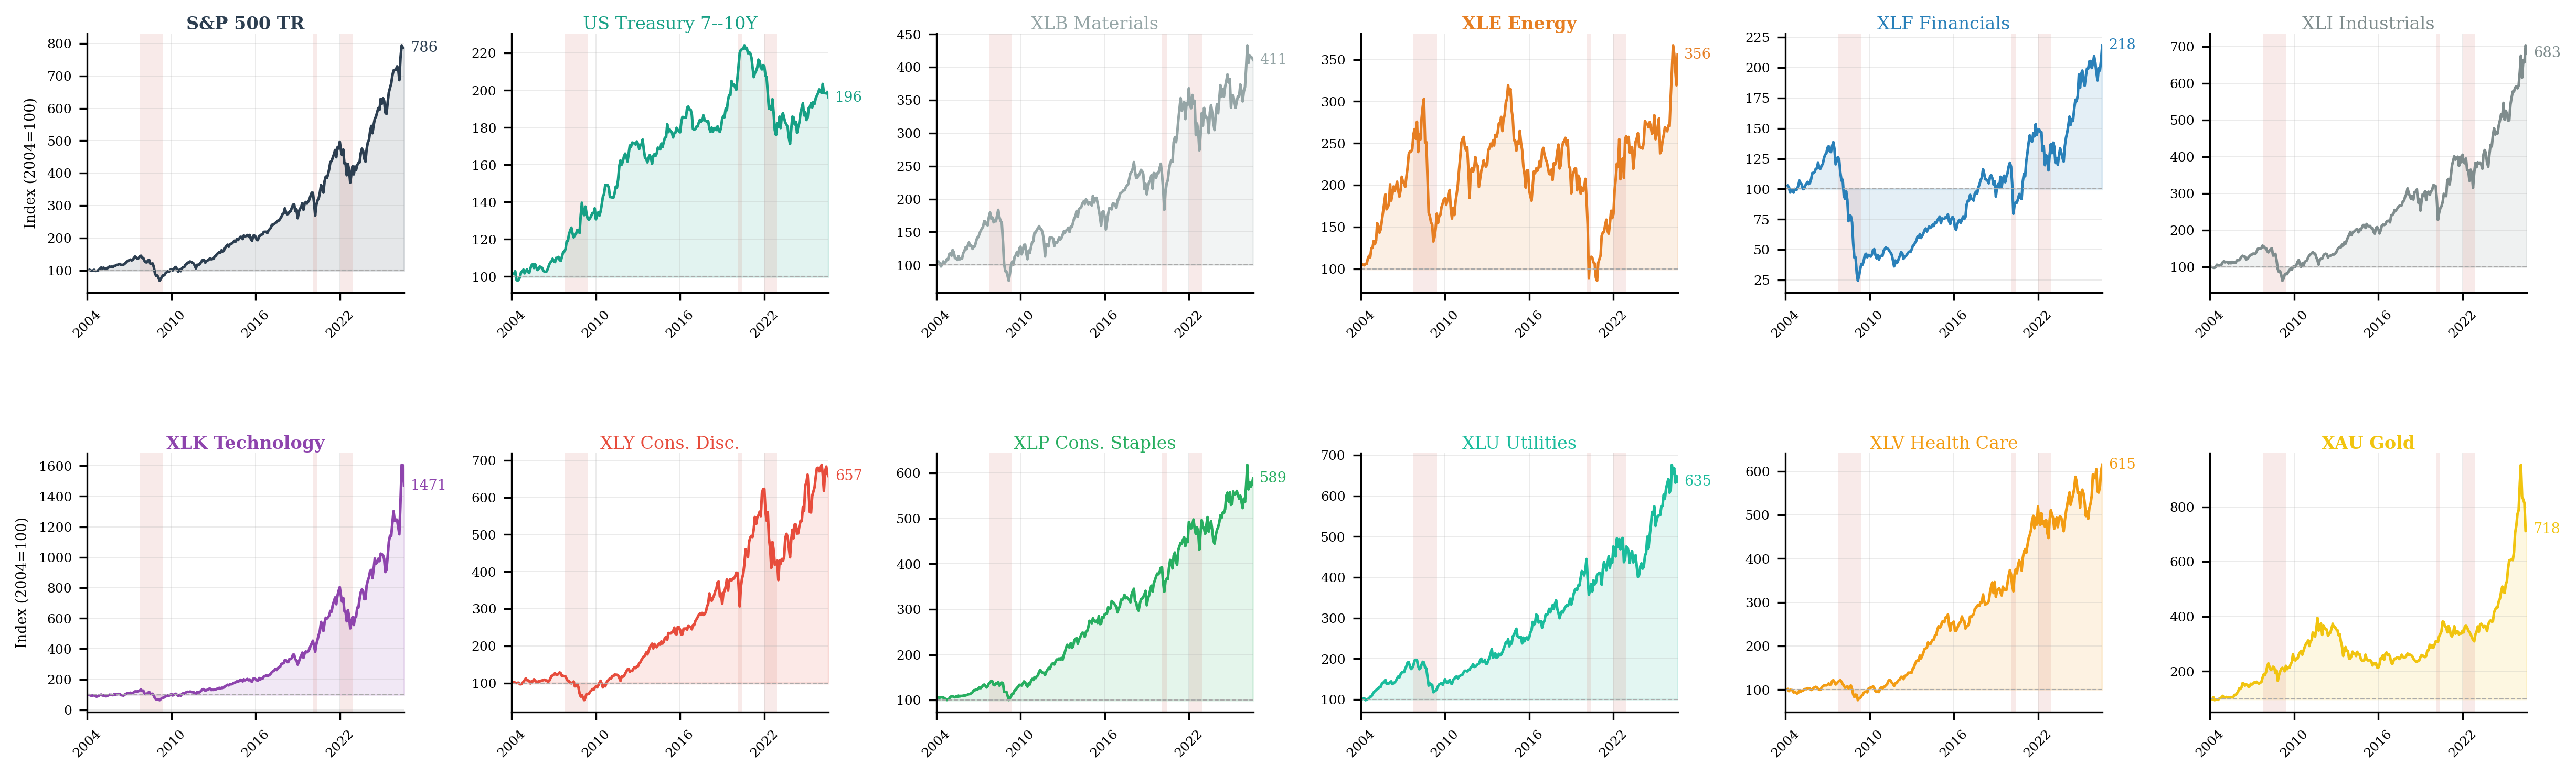
\includegraphics[width=0.96\linewidth]{figures/fig1_asset_price_levels}
  \caption{Cumulative price levels of the core and satellite assets, rebased to 100 at
           February 2004. Shaded regions mark the three crisis episodes inside the sample. Final index
           values are annotated at the right of each panel. XLK (Technology, 1471) and XAU
           (Gold, 718) are the highest-returning satellites over the full period, while
           XLE (Energy, 356) and XLF (Financials, 218) are the weakest cyclical performers,
           reflecting the post-2014 energy bear market and the persistent post-GFC
           underperformance of financials respectively.}
  \label{fig:price_levels}
\end{figure}

% ============================================================

\section{Model}
\label{sec:model}
% ============================================================

\subsection{Estimated Regimes}

The three-state model fitted on the 1999--2026 sample produces three economically
interpretable regimes. Three or more states are found to outperform two-state
specifications \cit{angtimm2012}{(Ang and Timmermann 2012)}, and the latent state is inferred from the
filtered probability recursion \cit{hamilton1989}{(Hamilton 1989)}. Regime~0 covers crisis periods including the dotcom crash of
2000--2002, the Global Financial Crisis of 2008--2009, the 2020 COVID-19 drawdown, and the
2022 rate shock. Regime~1 is a transitional state that appears around regime turning points.
Regime~2 captures the sustained bull markets of 2003--2007, 2010--2019, and 2020--2021. The
regime-conditional moments and the transition matrix are reported in
Tables~\ref{tab:summary_stats} and~\ref{tab:transition}, and the state-count comparison in
Table~\ref{tab:model_selection}.

\subsection{Model Selection and the Two-Stage Design Rationale}

\textbf{Figure~\ref{fig:regime_probs}} shows the one-step-ahead predictive regime probabilities over the full 2004--2026 backtest period. The bear regime (Regime~0, red) spikes sharply during the GFC, COVID-19, and the 2022 rate shock, consistent with the rolling window adapting toward elevated bear-regime probability during these episodes. The transitional regime (Regime~1, orange) dominates the 2010--2016 recovery period, consistent with the model's adaptive response to the 2010--2016 recovery.

\section{Scoring Engine and Allocation Layer}
\label{sec:preferences}
\label{sec:allocation}
% ============================================================

The framework scores candidate allocations rather than optimising over them. Solving the
constrained problem in Equation~\eqref{eq:optimisation} directly would require numerical
optimisation at every rebalance date, which is computationally demanding and, for
higher-moment utility, sensitive to moment estimation error on a non-convex objective surface.
Expected utility is instead approximated \cit{jondeau2006}{(Jondeau and Rockinger 2006)} by a Taylor
expansion around the moments of the portfolio return distribution,
Equation~\eqref{eq:taylor_utility}, which is closed-form and stays accurate under moderate
non-normality. 

Investors are assumed to prefer positive skewness and dislike excess kurtosis, a property
that holds for risk-averse utility generally rather than for specific parametric forms
\cit{scott1980}{(Scott and Horvath 1980)}. Three investor types are nested truncations of that expansion: the MV investor truncates at
the second order, the MVS investor adds the skewness term, and the MVK investor adds
kurtosis. Separating MVS from MVK is deliberate. It isolates which moment drives
any observed improvement, and because the two preferences impose conflicting demands on the
return distribution in some configurations, keeping them apart allows clean attribution. The
preference parameters are calibrated at the unconditional moments of the benchmark so that
each higher-moment term contributes approximately 20\% of the variance term
(Table~\ref{tab:calibration}).

The architecture is core-plus-satellite, chosen for compatibility with the standardised
mandate. Under structural breaks a rolling window is preferred to an expanding one \cit{pesaran2007}{(Pesaran and Timmermann 2007)}, so the HMM is refitted on the trailing 60 months at each rebalance date
and the filtered probabilities propagated through the transition matrix,
Equation~\eqref{eq:predictive}. The model does not forecast
returns directly \cit{ma2011}{(Ma et al. 2011)}: this predictive vector is the only input the scoring engine receives. The
engine enumerates every feasible combination of at most two satellites on a 5\% weight grid
subject to the sleeve cap and adopts the best only if it beats the untilted core by more than
the score improvement floor, a confidence threshold in the spirit of earlier work \cit{nystrup2015}{(Nystrup et al. 2015)}.
Otherwise the portfolio holds the passive core and the month is recorded as a NONE
observation.

\section{Allocation Tilts and Computational Elements}
\label{sec:tilts}
% ============================================================

One of the novel contributions of this study is the tilt mechanism governing how the
sample sector ETFs replace the securities in the core benchmark portfolio. Because we divided
the ETFs into two distinct business cycle styles, we adapted the tilt mechanism to reflect the
statistical properties of their return distributions in that context. We labelled six ETFs as
cyclical and four, including gold, as defensive. The cyclical ETFs replace the benchmark
pro-rata, keeping the 60:40 ratio intact, while the defensive ETFs replace only the equity leg.
In testing we found that the sensible order of implementation is cyclicals first and defensives
second, because only that ordering leaves the bond weight a function of the cyclical allocation
alone: it scales to $(1-\Sigma_{\mathrm{cyc}})\times 40\%$, with the defensive allocation absent
from the expression. Reversing the order makes the bond weight depend on both, so the rule that
defensive tilts never touch the bond block would hold only approximately. While this mechanism
is simple, the principle follows the separation between the model that
ranks opportunities and the rules that implement them \cit{grinold2000}{(Grinold and Kahn 2000)}.

The signal used for the volatility channel is a realised semivariance rather than a total
variance, because the leverage asymmetry is driven specifically by the downside component
of realised variance \cit{patton2015}{(Patton and Sheppard 2015)}, \cit{moreira2017}{(Moreira and Muir 2017)}. The correlation
channel is kept endogenous because macroeconomic fundamentals explain little of the
stock--bond correlation \cit{baele2010}{(Baele et al. 2010)}, and realised measures
remain model-free and tractable when aggregated from high-frequency data \cit{andersen2003}{(Andersen et al. 2003)}.

Small regimes are handled by shrinkage: whenever a regime holds fewer than twelve
observations inside the current five-year window its covariance is replaced by the pooled
window covariance, so the slow correlation layer is never represented by an unstable
estimate \cit{ledoit2004}{(Ledoit and Wolf 2004)}.

The three sizing mechanisms share a motivation. The upside of the regime signal was already
established, and what remained was protection against sudden drawdowns, and all three are organised
around the same bear-regime probability. Because they act on different parts of the portfolio,
funding, sleeve size and core composition, but respond to the same underlying state, they
compound rather than offset. That is why the downside metrics improve materially while the
upside capture is preserved.
Figure~\ref{fig:pipeline} sets out the full pipeline from data to portfolio weights and the
equations that govern it.

\input{figures/fig_pipeline}

\subsection{Satellite Universe and Regime Styles}

The ten candidate satellites are classified by their expected behaviour across the
bear-bull regime dimension. The nine sector ETFs are the same universe used by the closest antecedent to this study \cit{ma2011}{(Ma et al. 2011)}. Cyclical sectors, namely Energy (XLE), Technology (XLK), Financials
(XLF), Industrials (XLI), Materials (XLB), and Consumer Discretionary (XLY) are expected
to outperform in bull regimes and underperform in bear regimes. Defensive sectors, namely Consumer
Staples (XLP), Utilities (XLU), and Health Care (XLV), are expected to preserve value in
bear regimes and lag in bull regimes. Gold (XAU) is classified as a defensive satellite,
reflecting its historically low and regime-varying correlation with the equity market.
On the same SPDR universe gold's safe-haven role is found to be sector-specific
\cit{kinateder2024}{(Kinateder et al. 2024)}, which motivates treating it as a scored
candidate rather than a permanent strategic allocation.

\subsection{Conviction Scalar}

The applied satellite weight is not the scored weight. A conviction scalar modulates it by
regime certainty: cyclical satellites are scaled by $(1-p_{\text{bear}})$ and defensive
satellites, gold included, by $p_{\text{bear}}$. The full scored weight is therefore applied
only when the model is confident about the prevailing regime. When no regime clearly dominates,
the sleeve shrinks toward zero and the portfolio gravitates back to the passive core. The realised sleeve over
the full sample is shown in Figure~\ref{fig:satweights}.

\begin{figure}[t]
  \centering
  \includegraphics[width=0.96\linewidth]{figures/fig_satellite_weights_35_MVS}
  \caption{Monthly satellite allocation weights by sector (MVS investor, 35\% sleeve,
           score improvement floor 0.001, February 2004 -- July 2026). Shaded bands mark the
           three crisis episodes. Bold frames highlight the three satellites that carry the
           allocation: XLE through the 2004--2012 commodity cycle and again from 2022, XLK
           from 2018 onward, and XAU concentrated in the 2004--2012 and 2020--2026 stress
           periods. The defensive sectors (XLP, XLU, XLV) are selected only rarely, which is
           consistent with the displacement rule funding defensive tilts from the equity leg
           rather than from the whole core.}
  \label{fig:satweights}
\end{figure}

\section{Results}
\label{sec:results}
% ============================================================

\subsection{Headline Performance}

Table~\ref{tab:sensitivity_main} reports the two operating points against the benchmark, with the full sensitivity analysis across satellite sleeve
sizes and investor types over the 2004--2026 sample of 270 months. All figures are net of
transaction costs of five basis points per leg. Two configurations are carried forward as
reported operating points, both using the MVS investor and a score improvement floor of 0.001.

\input{figures/tab_sensitivity_main}

The 30\% configuration improves on the benchmark on every risk-adjusted metric reported,
including downside deviation, the one metric on which a return-seeking tilt would ordinarily
be expected to lose ground. The 35\% sleeve carries the highest Sharpe ratio in the grid, at
the cost of a downside deviation that now exceeds the benchmark.

We report two operating points rather than one because they answer different questions. The
30\% sleeve is the risk-managed configuration: it is the largest sleeve at which downside
deviation remains below the benchmark, so every risk-adjusted metric improves simultaneously
and the tilt cannot be said to have bought return by accepting more downside risk. The 35\%
sleeve is the peak risk-adjusted return, at the cost of a downside deviation that now exceeds
the benchmark. Choosing between them is a mandate decision rather than a statistical one, and
we leave it open deliberately. That the MVS investor is best or joint-best at every sleeve is
the more general result: adding a skewness term to the scoring function improves selection
against plain mean-variance across the whole grid, while the kurtosis-averse specification
does not, which suggests the gain comes from preferring asymmetry rather than from penalising
tail risk.

\subsection{Capture Asymmetry}

Up- and down-capture ratios are computed against the benchmark over months in which the
benchmark return is positive and negative respectively. At the 30\% sleeve the strategy
captures 102.8\% of benchmark upside and 88.8\% of benchmark downside, a capture spread of
0.140. At the 35\% sleeve the corresponding figures are 105.4\% and 89.3\%, a spread of 0.161.
Down-capture remains below 93\% at every sleeve size between 20\% and 45\%, while up-capture
exceeds 100\% from the 25\% sleeve upward.

This is the central claim of the paper: protection purchased without surrendering
participation. The distinction matters because a portfolio that simply holds less equity risk
cannot produce this pattern. A symmetric reduction in equity beta lowers participation in
rising months by roughly as much as it lowers exposure in falling ones, so both capture ratios
move together and the spread between them is left broadly unchanged. What is reported here is
the opposite: up-capture rises above 100\% while down-capture falls below 90\%, and the spread
widens with sleeve size. The asymmetry therefore has to originate in the conditioning layers
deciding \emph{when} defensive exposure is held, not in holding less risk on average. That is
the economic content of the two-stage separation. Selection preserves participation, and sizing
withdraws exposure only in the months when both the regime signal and the volatility signal
point to stress.

\subsection{Drawdown Episodes}

Performance is also evaluated conditional on benchmark drawdown episodes, defined as
peak-to-recovery windows in which the benchmark declines by more than five percent. Over the
2007--2010 episode, in which the benchmark reached a trough of $-30.6$\%, the strategy
outperforms by 10.4 percentage points at the 30\% sleeve and 11.1 points at the 35\% sleeve.
Over the February--June 2020 episode, with a benchmark trough of $-9.9$\%, the margins are 0.8
and 1.2 points. Over the 2022 rate shock, with a benchmark trough of $-20.7$\%, the strategy
underperforms the benchmark by 1.96 points at the 30\% sleeve and 2.81 points at the 35\%
sleeve, and this shortfall widens monotonically with sleeve size.

The Global Financial Crisis is the clearest case of the mechanism operating as designed. The
episode was long enough for the regime model to identify the bear state and persistent enough
for the displacement rule to hold the bond block intact while the sleeve rotated defensive,
and the two channels compounded over the full drawdown. COVID-19 produces a much smaller
margin for the opposite reason: the decline and recovery were compressed into weeks, and a
monthly rebalancing schedule can only respond to an episode that outlasts its decision
interval.

The 2022 result is the exception, and the reason is mechanical. The volatility channel did
detect the episode, with seven of the eleven decision months armed, so the shortfall is not a
detection failure. It reflects where the de-risking goes: into the core, whose bond block was
itself falling in a rate-driven drawdown. That the shortfall widens with sleeve size fits that
reading, since a larger sleeve moves more weight into the declining asset. A framework
conditioned on equity stress is least effective when equities and bonds fall together.

\subsection{Holding-Period Analysis}

Because a monthly rebalanced strategy is held over horizons considerably longer than a month,
performance is also evaluated across overlapping holding periods.
Table~\ref{tab:rolling_horizon} reports the full distribution of outcomes. At the 35\% sleeve
the strategy outperforms the benchmark in 50.7\% of overlapping one-month windows, 59.0\% of
three-month windows, 60.0\% of six-month windows, 67.2\% of one-year windows, 86.4\% of
three-year windows and 95.7\% of five-year windows.

\begin{table}[t]
\centering
\caption{Distribution of Outcomes by Holding Period (35\% Sleeve, MVS Investor)}
\label{tab:rolling_horizon}
\setlength{\tabcolsep}{5pt}
\footnotesize
\resizebox{\textwidth}{!}{%
\begin{tabular}{lrr rr rr rr rr}
\toprule
 & & & \multicolumn{2}{c}{\textbf{Mean return (\%)}} & \multicolumn{2}{c}{\textbf{Std.\ dev.\ (\%)}}
 & \multicolumn{2}{c}{\textbf{Skewness}} & \multicolumn{2}{c}{\textbf{Windows with a loss (\%)}} \\
\cmidrule(lr){4-5}\cmidrule(lr){6-7}\cmidrule(lr){8-9}\cmidrule(lr){10-11}
\textbf{Holding period} & \textbf{Windows} & \textbf{Hit rate (\%)}
 & \textbf{Strat.} & \textbf{Bench.} & \textbf{Strat.} & \textbf{Bench.}
 & \textbf{Strat.} & \textbf{Bench.} & \textbf{Strat.} & \textbf{Bench.} \\
\midrule
1 month   & 270 & 50.7 &  0.81 &  0.66 &  2.69 &  2.61 & $-$0.78 & $-$0.66 & 31.1 & 31.9 \\
3 months  & 268 & 59.0 &  2.42 &  1.98 &  4.33 &  4.24 & $-$0.91 & $-$0.87 & 20.5 & 25.4 \\
6 months  & 265 & 60.0 &  4.94 &  4.02 &  6.32 &  6.21 & $-$1.21 & $-$1.30 & 16.2 & 17.7 \\
1 year    & 259 & 67.2 & 10.10 &  8.25 &  9.19 &  9.11 & $-$1.29 & $-$1.36 & 10.4 & 12.0 \\
3 years   & 235 & 86.4 & 31.89 & 25.51 & 14.35 & 15.67 & \phantom{$-$}0.10 & $-$0.36 & \textbf{0.0} & 10.6 \\
5 years   & 211 & 95.7 & 57.79 & 45.69 & 16.77 & 20.36 & \phantom{$-$}0.39 & $-$0.13 & \textbf{0.0} &  1.4 \\
\bottomrule
\end{tabular}}
\begin{minipage}{\linewidth}
\vspace{4pt}\footnotesize
\textit{Notes:} Overlapping windows slid one month at a time across the 2004--2026 sample,
35\% satellite sleeve, MVS investor, score improvement floor 0.001, net of transaction costs.
Each window pairs the strategy against the benchmark realised over the \emph{same} window.
Hit rate is the share of windows in which the strategy return exceeds the benchmark return.
Windows with a loss is the share of windows ending in a negative compounded return.
\end{minipage}
\end{table}



The monotone rise in hit rate with horizon is the signature we would expect from a strategy
whose edge is concentrated in stress episodes rather than spread evenly across months. In a
typical month the model holds a tilt that neither helps nor hurts materially, so the one-month
result sits close to a coin flip. As the window lengthens it becomes progressively more likely
to contain one of the episodes in which the conditioning layers actually act, and the hit rate
rises accordingly.

\subsection{Turnover and Implementation}

All results are net of transaction costs of five basis points per leg, charged on two-way
turnover at each rebalancing date. The strategy is active in 267 of 270 months at the 30\%
sleeve and 269 at the 35\% sleeve, with average turnover of 24.5\% and 28.1\% in those months.
That is modest for a monthly strategy on instruments of this liquidity, and because every
figure is already net of costs the result is robust to the cost assumption rather than
dependent on it. Capacity and market impact at institutional size are not tested here. The
score improvement floor behaves as intended. It blocks a tilt whenever no candidate improves on
the untilted core by enough to justify the trade, which happens most often at small sleeve
sizes, where the available tilts are themselves small. The share of months returned to the
passive core for this reason falls steadily from 7.4\% at a 20\% sleeve to zero at 40\% and
above. The floor therefore screens out marginal tilts rather than holding the strategy back.


\section{Conclusion}
\label{sec:conclusion}
% ============================================================

This paper develops and empirically evaluates a regime-aware tactical allocation framework
for the equity sleeve of a 60/40 balanced portfolio. The framework combines a three-state
Hidden Markov Model for regime identification, a sector ETF and gold satellite universe, a
Taylor-expanded expected utility scoring function accommodating three investor preference
types, and a rolling 60-month estimation window that lets the model adapt to structural
breaks in sector leadership. The goal was straightforward: improve on a buy-and-hold
benchmark in a context constrained by the challenges facing passive wealth management.

The contribution is novel in its simplicity and operational feasibility. The model does not
forecast returns directly, but rather uses a one-step-ahead predictive probability as its
only signal. It does not involve a complex optimisation, but rather scores candidate
portfolios using the same expected-utility equations an optimiser would work from. Every
input is endogenous, drawn from the return series themselves and their descriptive
statistics. Because each stage of the model is defined to do one job and is kept separate
from the others, the layers compound rather than interfere. At a 35\% sleeve the strategy
captures 105\% of the benchmark's upside while taking only 89\% of its downside. A portfolio
that simply held less equity risk could not produce that pattern, since it would lower both
figures together. The asymmetry is what the design was built for, and it is where the layers
show they are coherent in both motivation and application.

The result also holds whenever an investor happens to start. The model beats the benchmark at
every holding period tested, and at three and five years there is no window in which an
investor ends at a loss. That the MVS configuration outperforms both MV and MVK suggests it is
the preference for positive skewness, rather than the penalty on tail risk, that is being
rewarded.

Future work could test the framework in other geographical settings, where the investor's
mandate is regionally motivated. One example would be a Eurostoxx total return index paired
with a German Bund or a French OAT. The core itself could differ, depending on the investor's
risk appetite and investment policy statement. The sizing signal is the clearest candidate for
improvement, since it is least effective when equities and bonds are highly correlated and the
market is in turmoil, as in the 2022 rate and inflation shock. The model could also be tested
against a more demanding benchmark built from the strong risk-adjusted periods of individual
sectors, such as energy in the early 2000s or technology after 2016.

Despite the concrete setting in which this study has been developed, we believe the framework
could be deployed in various multi-asset contexts. Scaling an exposure by a regime probability
is not specific to a satellite sleeve. The same mechanism could be put to work in a broader
dynamic risk management setting, where exposure limits follow the estimated regime
probabilities rather than being held fixed.

\section*{References}
\addcontentsline{toc}{section}{References}
% ============================================================

\begin{description}[leftmargin=2em, itemsep=2pt]

\new{\item \reftgt{andersen2003} Andersen, T.G., Bollerslev, T., Diebold, F.X. and Labys, P. (2003). Modeling and
  forecasting realized volatility. \textit{Econometrica}, 71(2), 579--625.}

\item \reftgt{angtimm2012} Ang, A. and Timmermann, A. (2012). Regime changes and financial markets.
  \textit{Annual Review of Financial Economics}, 4, 313--337.


\new{\item \reftgt{baele2010} Baele, L., Bekaert, G. and Inghelbrecht, K. (2010). The determinants of stock and
  bond return comovements. \textit{Review of Financial Studies}, 23(6), 2374--2428.}

\new{\item \reftgt{grinold2000} Grinold, R.C. and Kahn, R.N. (2000). \textit{Active Portfolio Management: A
  Quantitative Approach for Producing Superior Returns and Controlling Risk}, 2nd ed.
  McGraw-Hill.}

\item \reftgt{hamilton1989} Hamilton, J.D. (1989). A new approach to the economic analysis of nonstationary time
  series and the business cycle. \textit{Econometrica}, 57(2), 357--384.

\item \reftgt{jondeau2006} Jondeau, E. and Rockinger, M. (2006). Optimal portfolio allocation under higher
  moments. \textit{European Financial Management}, 12(1), 29--55.

\item \reftgt{kinateder2024} Kinateder, H., Gurrib, I. and Choudhury, T. (2024). Navigating crises: Gold's role as a safe haven for U.S. sectors. \textit{Finance Research Letters}, 69, 106210.

\new{\item \reftgt{ledoit2004} Ledoit, O. and Wolf, M. (2004). Honey, I shrunk the sample covariance matrix.
  \textit{Journal of Portfolio Management}, 30(4), 110--119.}

\item \reftgt{ma2011}Ma, Y., MacLean, L., Xu, K. and Zhao, Y. (2011). A portfolio optimisation model with
  regime-switching risk factors for sector exchange traded funds.
  \textit{Pacific-Basin Finance Journal}, 19(2), 206--226.


\new{\item \reftgt{moreira2017} Moreira, A. and Muir, T. (2017). Volatility-managed portfolios.
  \textit{Journal of Finance}, 72(4), 1611--1644.}

\item \reftgt{nystrup2015} Nystrup, P., Hansen, B.W., Madsen, H. and Lindstr{\"o}m, E. (2015). Regime-based
  versus static asset allocation: Letting the data speak.
  \textit{Journal of Portfolio Management}, 42(1), 103--109.

\new{\item \reftgt{patton2015} Patton, A.J. and Sheppard, K. (2015). Good volatility, bad volatility: signed jumps
  and the persistence of volatility. \textit{Review of Economics and Statistics}, 97(3),
  683--697.}

\item \reftgt{pesaran2007} Pesaran, M.H. and Timmermann, A. (2007). Selection of estimation window in the
  presence of breaks. \textit{Journal of Econometrics}, 137(1), 134--161.

\item \reftgt{pwc2025}PwC (2025). \textit{Asset and Wealth Management Revolution 2025}.
  PricewaterhouseCoopers.

\item \reftgt{scott1980} Scott, R.C. and Horvath, P.A. (1980). On the direction of preference for moments of
  higher order than the variance. \textit{Journal of Finance}, 35(4), 915--919.

\end{description}

\clearpage
% ============================================================
\appendix
\section{Appendix}
\label{sec:appendix_all}
% ============================================================

\subsection*{A.1 Full sensitivity analysis}

\input{figures/tab_sensitivity_new}

\subsection*{A.2 Data, model selection and calibration}

\begin{table}[H]
\centering
\caption{Descriptive Statistics for Monthly Log Returns, Full Sample (Feb 2004 -- Jul 2026)}
\label{tab:data_stats}
\setlength{\tabcolsep}{4pt}
\footnotesize
\resizebox{\textwidth}{!}{%
\begin{tabular}{lrrrrrrr}
\toprule
\textbf{Asset} & \textbf{Ann.\ Mean (\%)} & \textbf{Ann.\ Vol (\%)} & \textbf{Sharpe} & \textbf{Skewness} & \textbf{Exc.\ Kurt.} & \textbf{Min (\%)} & \textbf{Max (\%)} \\
\midrule
\multicolumn{8}{l}{\textit{Core assets}} \\[2pt]
S\&P 500 TR        & 10.30 & 14.71 & 0.530 & $-$0.757 & 1.759 & $-$18.39 & 12.06 \\
LT Bond (7--10y)   &  3.20 &  6.39 & 0.110 & \phantom{$-$}0.065 & 0.857 & $-$4.80  & 7.69  \\
\midrule
\multicolumn{8}{l}{\textit{Cyclical sector satellites}} \\[2pt]
XLB Materials      &  8.27 & 19.67 & 0.293 & $-$0.558 & 1.843 & $-$25.35 & 15.99 \\
XLE Energy         &  9.19 & 26.00 & 0.257 & $-$0.652 & 4.402 & $-$42.12 & 26.82 \\
XLF Financials     &  5.92 & 21.54 & 0.159 & $-$1.120 & 4.147 & $-$30.38 & 19.72 \\
XLI Industrials    & 10.29 & 18.38 & 0.424 & $-$0.720 & 2.201 & $-$20.61 & 16.61 \\
XLK Technology     & 13.74 & 18.60 & 0.604 & $-$0.240 & 0.648 & $-$17.58 & 18.24 \\
XLY Cons.\ Disc.   & 10.11 & 18.51 & 0.411 & $-$0.238 & 1.365 & $-$19.40 & 17.30 \\
\midrule
\multicolumn{8}{l}{\textit{Defensive sector satellites}} \\[2pt]
XLP Cons.\ Staples &  8.61 & 11.84 & 0.516 & $-$0.591 & 1.147 & $-$13.48 & 9.94  \\
XLU Utilities      &  9.28 & 14.29 & 0.474 & $-$0.790 & 0.954 & $-$13.93 & 10.03 \\
XLV Health Care    &  9.04 & 13.68 & 0.478 & $-$0.404 & 0.440 & $-$13.23 & 11.86 \\
\midrule
\multicolumn{8}{l}{\textit{Commodity satellite}} \\[2pt]
XAU Gold           & 10.26 & 17.10 & 0.454 & $-$0.252 & 0.645 & $-$18.50 & 12.49 \\
\bottomrule
\end{tabular}}
\begin{minipage}{\linewidth}
\vspace{4pt}\footnotesize
\textit{Notes:} Monthly log returns from the allocation backtest period (February 2004 -- July 2026, $T=270$ monthly observations). Annual mean and volatility obtained by multiplying monthly mean by 12 and monthly standard deviation by $\sqrt{12}$. Sharpe ratio uses an approximate average 1-month T-bill rate of 2.5\% per annum as the risk-free rate. Skewness and excess kurtosis use Fisher's definition. All nine sector ETF returns obtained via Yahoo Finance API; XAU obtained from Bloomberg; LT Bond = \texttt{LT09TRUU} Bloomberg US Treasury 7--10 Year index.
\end{minipage}
\end{table}

\begin{table}[H]
\centering
\caption{Pairwise Correlation Matrix of Monthly Log Returns (Feb 2004 -- Jul 2026)}
\label{tab:correlations}
\setlength{\tabcolsep}{3.5pt}
\footnotesize
\resizebox{\textwidth}{!}{%
\begin{tabular}{lrrrrrrrrrrrr}
\toprule
 & \textbf{SP500} & \textbf{Bond} & \textbf{XLB} & \textbf{XLE} & \textbf{XLF} & \textbf{XLI} & \textbf{XLK} & \textbf{XLY} & \textbf{XLP} & \textbf{XLU} & \textbf{XLV} & \textbf{XAU} \\
\midrule
SP500 & 1.00 & $-$0.05 & 0.85 & 0.60 & 0.84 & 0.91 & 0.89 & 0.90 & 0.71 & 0.49 & 0.74 & 0.10 \\
Bond  &      & 1.00 & $-$0.10 & $-$0.25 & $-$0.16 & $-$0.09 & $-$0.03 & $-$0.02 & 0.12 & 0.23 & 0.05 & 0.33 \\
XLB   &      &      & 1.00 & 0.66 & 0.74 & 0.87 & 0.68 & 0.76 & 0.63 & 0.44 & 0.65 & 0.25 \\
XLE   &      &      &      & 1.00 & 0.54 & 0.61 & 0.40 & 0.46 & 0.41 & 0.32 & 0.40 & 0.13 \\
XLF   &      &      &      &      & 1.00 & 0.83 & 0.61 & 0.75 & 0.58 & 0.33 & 0.62 & $-$0.03 \\
XLI   &      &      &      &      &      & 1.00 & 0.73 & 0.82 & 0.69 & 0.46 & 0.67 & 0.07 \\
XLK   &      &      &      &      &      &      & 1.00 & 0.81 & 0.51 & 0.36 & 0.54 & 0.04 \\
XLY   &      &      &      &      &      &      &      & 1.00 & 0.58 & 0.35 & 0.60 & 0.04 \\
XLP   &      &      &      &      &      &      &      &      & 1.00 & 0.61 & 0.69 & 0.16 \\
XLU   &      &      &      &      &      &      &      &      &      & 1.00 & 0.45 & 0.24 \\
XLV   &      &      &      &      &      &      &      &      &      &      & 1.00 & 0.11 \\
XAU   &      &      &      &      &      &      &      &      &      &      &      & 1.00 \\
\bottomrule
\end{tabular}}
\begin{minipage}{\linewidth}
\vspace{4pt}\footnotesize
\textit{Notes:} Pearson correlations of monthly log returns. Several features of this matrix motivate the satellite selection logic. XAU (gold) has near-zero correlation with every sector ETF (between $-0.03$ and $0.25$) and a mildly positive correlation with bonds (0.33), so it diversifies the equity leg without duplicating the bond block. XLE (energy) has the lowest correlation with the S\&P~500 among the cyclical sectors (0.60), explaining its frequent selection during the 2004--2009 commodity supercycle. XLU (utilities) has the lowest sector-to-S\&P~500 correlation overall (0.49), consistent with its defensive classification. Bond--equity correlation is $-0.05$ unconditionally but varies substantially across regimes.
\end{minipage}
\end{table}

\begin{table}[htbp]
\centering
\caption{Summary Statistics for Monthly Excess Log Returns by HMM Regime}
\label{tab:summary_stats}
\setlength{\tabcolsep}{4pt}
\footnotesize
\resizebox{\textwidth}{!}{%
\begin{tabular}{llrrrrrrc}
\toprule
\textbf{Regime} & \textbf{Asset}
  & \textbf{Mean} & \textbf{Std Dev} & \textbf{Skew.}
  & \textbf{Exc.\ Kurt.} & \textbf{Min} & \textbf{Max} & \textbf{Corr.} \\
\midrule
\multicolumn{9}{l}{\textit{Return figures in \% per month; Corr.\ = conditional Pearson correlation between S\&P 500 TR and LT Bond.}} \\[2pt]
\midrule
\multirow{2}{*}{\shortstack[l]{\textbf{Regime 0: Bear}\\[1pt]\textit{N\,=\,20 (6.0\%)}}}
  & S\&P 500 TR  & $-$2.916 & 7.949 & \phantom{$-$}0.115 & $-$0.972 & $-$18.466 & \phantom{$-$}9.130 & \multirow{2}{*}{\phantom{$-$}0.28} \\
  & LT Bond      & $-$0.523 & 3.443 & \phantom{$-$}0.772 & $-$0.174 & $-$4.993  & \phantom{$-$}7.657 &  \\[6pt]
\midrule
\multirow{2}{*}{\shortstack[l]{\textbf{Regime 1: Transitional}\\[1pt]\textit{N\,=\,114 (34.4\%)}}}
  & S\&P 500 TR  & $-$0.293 & 5.204 & $-$0.106 & $-$0.431 & $-$13.303 & \phantom{$-$}12.062 & \multirow{2}{*}{$-$0.59} \\
  & LT Bond      & \phantom{$-$}0.727 & 1.700 & $-$0.091 & $-$0.479 & $-$3.519  & \phantom{$-$}4.747  &  \\[6pt]
\midrule
\multirow{2}{*}{\shortstack[l]{\textbf{Regime 2: Bull}\\[1pt]\textit{N\,=\,197 (59.5\%)}}}
  & S\&P 500 TR  & \phantom{$-$}1.358 & 2.911 & $-$0.070 & $-$0.030 & $-$6.139  & \phantom{$-$}9.688 & \multirow{2}{*}{\phantom{$-$}0.20} \\
  & LT Bond      & $-$0.122 & 1.624 & $-$0.380 & \phantom{$-$}0.790 & $-$5.915  & \phantom{$-$}4.001 &  \\[6pt]
\midrule
\multirow{2}{*}{\shortstack[l]{\textbf{Full Sample}\\[1pt]\textit{N\,=\,331 (100\%)}}}
  & S\&P 500 TR  & \phantom{$-$}0.531 & 4.394 & $-$0.628 & \phantom{$-$}1.046 & $-$18.466 & \phantom{$-$}12.062 & \multirow{2}{*}{$-$0.12} \\
  & LT Bond      & \phantom{$-$}0.147 & 1.850 & $-$0.034 & \phantom{$-$}0.845 & $-$5.915  & \phantom{$-$}7.657  &  \\
\bottomrule
\end{tabular}}
\begin{minipage}{\linewidth}
\vspace{4pt}\footnotesize
\textit{Notes:} Excess log returns $= \log(1+r_t) - \log(1+r_{f,t})$; $r_{f,t}$ = one-month T-bill rate.
Regime assignments: Viterbi hard-state sequence, best-seed HMM over 25 random initialisations
(seed\,=\,6, log-likelihood\,=\,1469.57). Regimes are ordered by ascending mean equity excess
return, so Regime~0 is always the bear state. Skewness and excess kurtosis follow Fisher's
definition. Sample: January 1999 -- July 2026 ($T = 331$ monthly observations).
The bond--equity correlation is \emph{positive} in the bear regime ($+0.28$): the twenty
bear-state months include the 2022 rate shock, in which equities and bonds fell together. The
strongest diversification appears in the transitional regime ($-0.59$), not in the bear state.
\end{minipage}
\end{table}

\begin{table}[htbp]
\centering
\caption{HMM Transition Probability Matrix and Regime Persistence (1999--2026)}
\label{tab:transition}
\setlength{\tabcolsep}{8pt}
\small
\resizebox{\textwidth}{!}{%
\begin{tabular}{lcccc}
\toprule
\textbf{From $\backslash$ To} & \textbf{Regime 0 (Bear)} & \textbf{Regime 1 (Trans.)} & \textbf{Regime 2 (Bull)} & \textbf{Exp.\ Duration} \\
\midrule
Regime 0 (Bear)         & 0.887 & 0.000 & 0.113 & 8.9 months  \\
Regime 1 (Transitional) & 0.012 & 0.939 & 0.048 & 16.5 months \\
Regime 2 (Bull)         & 0.004 & 0.042 & 0.954 & 21.7 months \\
\bottomrule
\end{tabular}}
\begin{minipage}{\linewidth}
\vspace{4pt}\footnotesize
\textit{Notes:} Estimated on the full January 1999 -- July 2026 sample ($T=331$), best seed over
25 random initialisations. Each row sums to one; entries below 0.0005 are shown as 0.000.
Expected duration $=1/(1-p_{kk})$. Regime~2 (Bull) is the most persistent state at 21.7 months.
This matrix is descriptive of the full sample. The backtest never uses it: predictive
probabilities are formed from a transition matrix re-estimated inside each trailing 60-month
window.
The zero entry $p_{01}$ implies the model never transitions directly from the bear state into
the transitional state: recovery from a crisis runs through the bull state.
\end{minipage}
\end{table}

\begin{table}[htbp]
\centering
\caption{Model Selection: Log-Likelihood, AIC and BIC for $K = 2, 3, 5$ States}
\label{tab:model_selection}
\setlength{\tabcolsep}{8pt}
\small
\begin{tabular}{lrrrrrr}
\toprule
\textbf{States} & \textbf{Log-lik.} & \textbf{Params} & \textbf{AIC} & \textbf{BIC}
  & \textbf{Avg.\ dur.\ (mo)} & \textbf{Min.\ regime frac.} \\
\midrule
$K = 2$ & 1451.80 & 13 & $-$2877.60 & $-$2828.17 & 10.4 & 0.221 \\
$K = 3$ & \textbf{1469.57} & 23 & $\mathbf{-}$\textbf{2893.14} & $-$2805.69 & 15.7 & 0.060 \\
$K = 5$ & 1490.42 & 49 & $-$2882.85 & $-$2696.54 & 6.6 & 0.015 \\
\bottomrule
\end{tabular}
\begin{minipage}{\linewidth}
\vspace{4pt}\footnotesize
\textit{Notes:} Best log-likelihood across 25 random seeds for each $K$. Free parameters:
$(K^2-K)$ transition probabilities $+ K\times 2$ means $+ K\times 3$ unique covariance entries $+ (K-1)$
initial state probabilities. AIC $= -2\mathcal{L} + 2p$; BIC $= -2\mathcal{L} + p\ln T$, $T=331$.
$K=3$ is selected: it has the best AIC ($-2893.14$) and adequate minimum regime fraction (6.0\%). $K=2$ has the best BIC but collapses the bear and transitional states into one, losing economic interpretability. $K=5$ achieves the highest log-likelihood but produces a degenerate regime with only 1.5\% of observations and an average duration of 6.6 months, consistent with overfitting. Bold = selected specification.
\end{minipage}
\end{table}

\begin{table}[H]
\centering
\caption{Score Term Calibration at Benchmark Unconditional Moments}
\label{tab:calibration}
\setlength{\tabcolsep}{6pt}
\small
\begin{tabular}{llrrr}
\toprule
\textbf{Score term} & \textbf{Formula} & \textbf{Value}
  & \textbf{\% of mean} & \textbf{\% of variance} \\
\midrule
Mean return      & $\mu_p$                   & 0.006486 & 100\% (primary) & ---  \\
Variance penalty & $\lambda \cdot \sigma^2$  & 0.002034 & 31\%              & 100\% (anchor) \\
Skewness term    & $\gamma \cdot |\text{sk}|$& 0.000424 & 7\%               & 21\% (mod.\ $\gamma$) \\
Kurtosis term    & $\delta \cdot |\kappa_e|$ & 0.000421 & 6\%               & 21\% (mod.\ $\delta$) \\
\bottomrule
\end{tabular}
\begin{minipage}{\linewidth}
\vspace{4pt}\footnotesize
\textit{Note:} Benchmark 60/40 moments over the full sample (Feb 2004 -- Jul 2026,
$T=270$): $\sigma^2=0.000678$, skew $=-0.74$, excess kurtosis $=2.03$, $\mu=0.006486$.
Preference parameters are held at their original calibration and are \emph{not} re-fitted to
the extended sample: $\lambda=3$, $\gamma_{\text{cons}} = 0.000431$,
$\gamma_{\text{mod}} = 0.000574$, $\delta_{\text{mod}} = 0.000207$. The higher-moment terms
therefore now sit at 21\% of the variance term rather than the 20\% originally targeted, a
difference that leaves the ranking of candidates unaffected.
\end{minipage}
\end{table}


\begin{sidewaysfigure}[p]
  \centering
  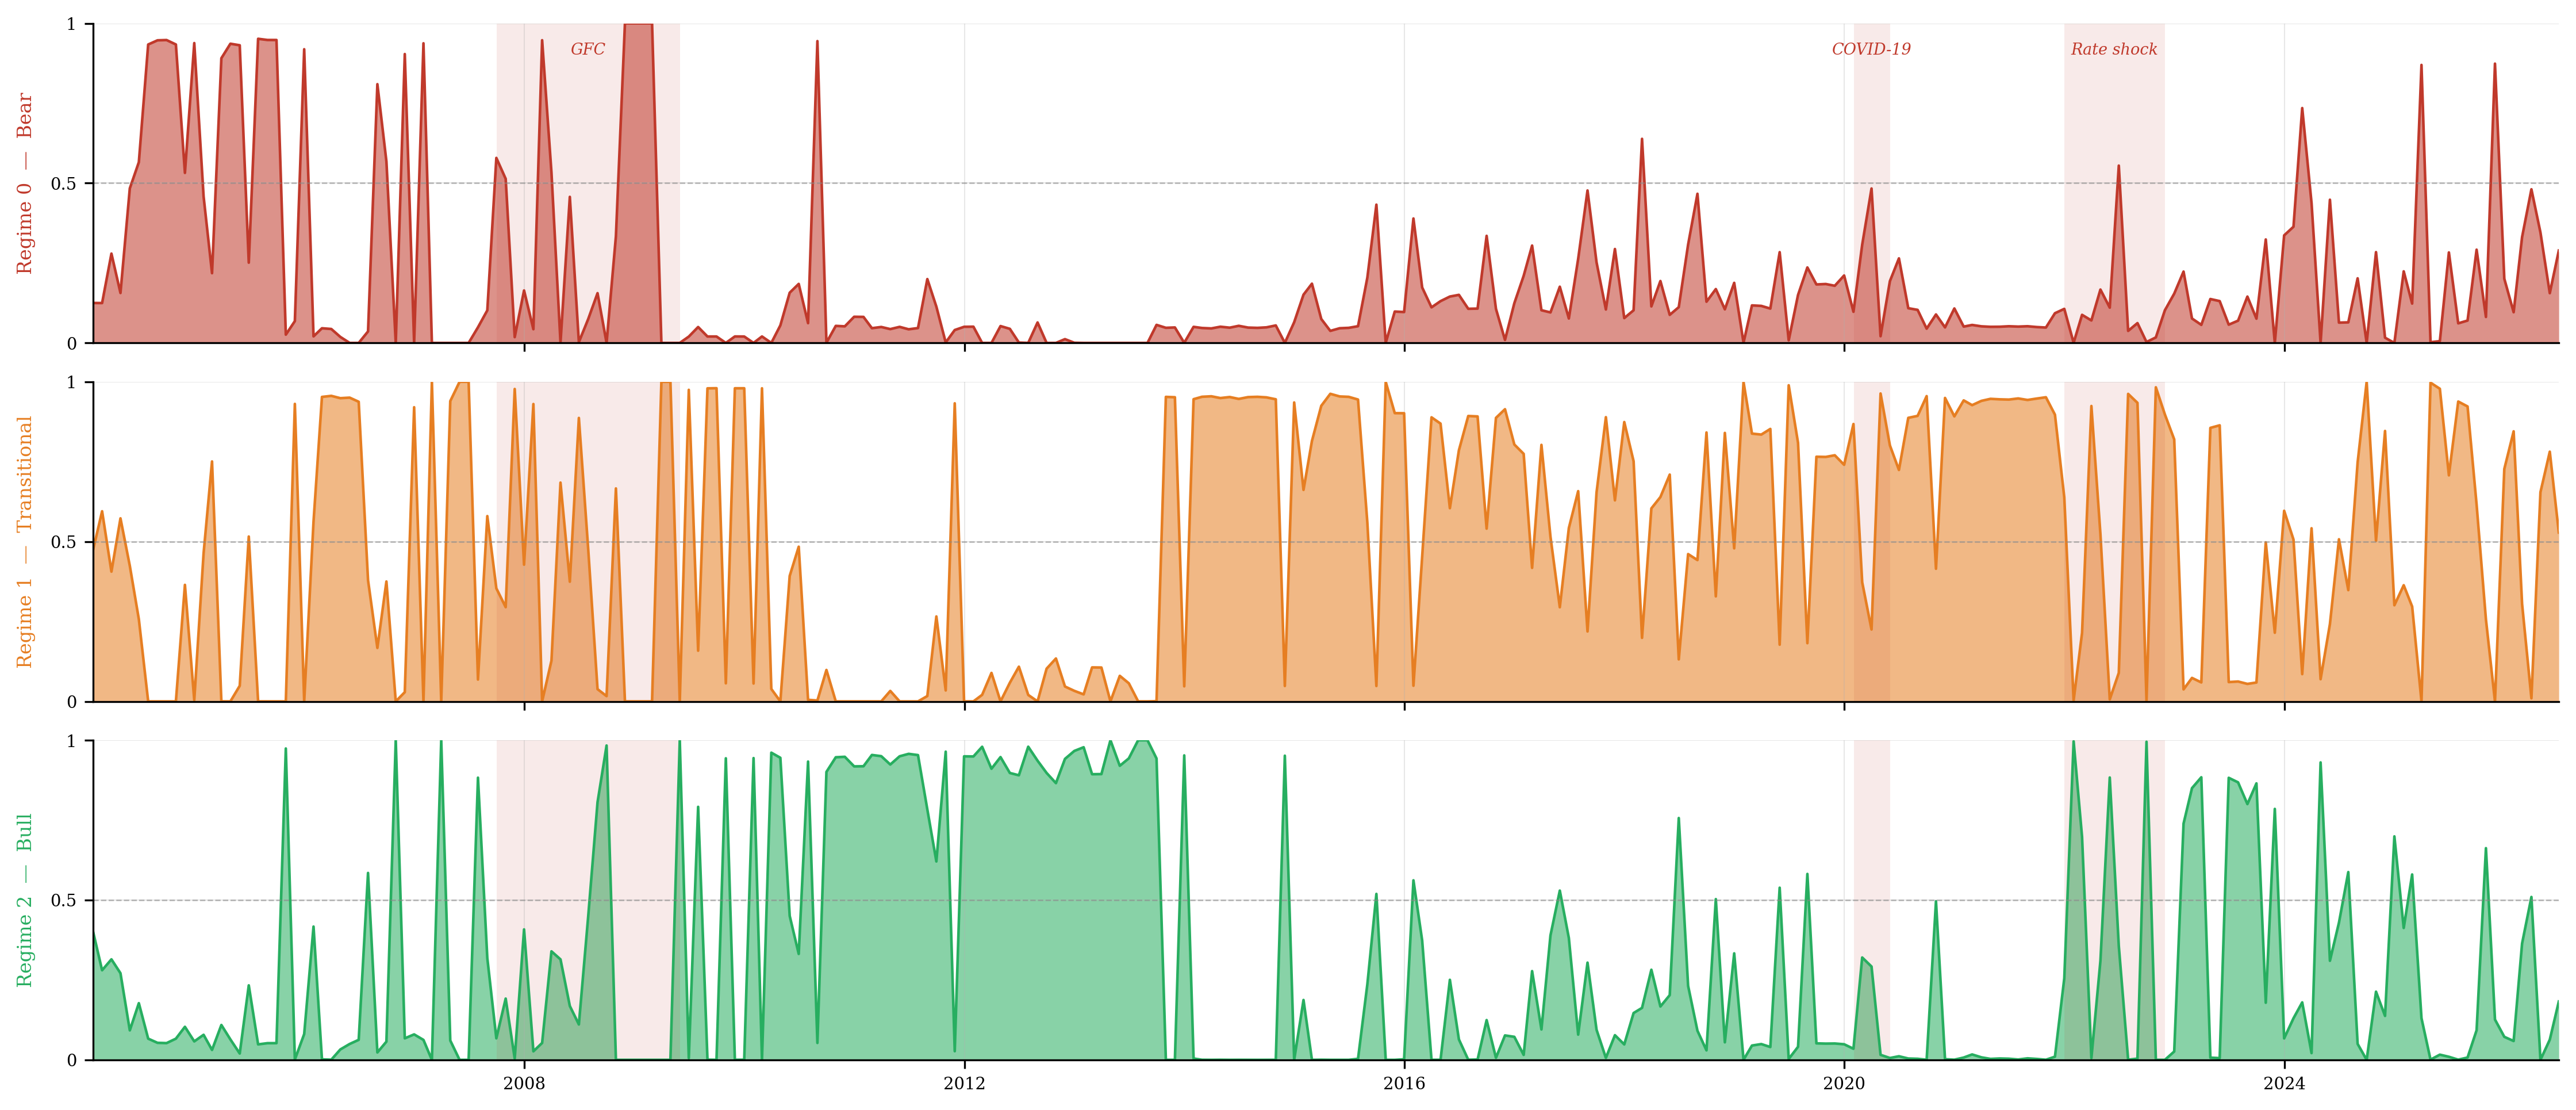
\includegraphics[width=\linewidth]{figures/fig2_regime_probabilities}
  \caption{One-step-ahead predictive regime probabilities from the three-state HMM
           (rolling 60-month window, February 2004 -- July 2026). Each panel shows the
           probability of one regime; shaded bands mark the three crisis episodes inside
           the backtest window.}
  \label{fig:regime_probs}
\end{sidewaysfigure}

\clearpage
\subsection*{A.3 Supporting specifications}

The numbered model equations referenced in the text are stated in
Figure~\ref{fig:pipeline}. The supporting specifications are collected here.

\begin{equation}
  \mathbf{Y}_t \mid S_t = k \;\sim\; \mathcal{N}\!\left(\boldsymbol{\mu}_k,\,
  \boldsymbol{\Sigma}_k\right)
  \label{eq:hmm_emission}
\end{equation}

\begin{equation}
  \xi_{t|t}(k) = \Pr\!\left(S_t = k \mid \mathbf{Y}_1,\ldots,\mathbf{Y}_t;\,
  \boldsymbol{\theta}\right)
  \label{eq:filtered}
\end{equation}

\begin{equation}
  \xi_{t|t-1}(k) = \sum_{j} \xi_{t-1|t-1}(j)\, p_{jk}
  \label{eq:prediction}
\end{equation}

\begin{equation}
  f(\mathbf{Y}_t \mid S_t = k;\,\boldsymbol{\theta})
  = \frac{1}{(2\pi)^{n/2}\,|\boldsymbol{\Sigma}_k|^{1/2}}
    \exp\!\left(-\tfrac{1}{2}
    (\mathbf{Y}_t - \boldsymbol{\mu}_k)^\prime
    \boldsymbol{\Sigma}_k^{-1}
    (\mathbf{Y}_t - \boldsymbol{\mu}_k)
    \right)
  \label{eq:emission_density}
\end{equation}

\begin{equation}
  \alpha_t(k) = p(\mathbf{Y}_1,\ldots,\mathbf{Y}_t,\, S_t = k;\,\boldsymbol{\theta})
  \label{eq:forward_var}
\end{equation}

\begin{equation}
  \alpha_1(k) = \pi_{0,k} \cdot f(\mathbf{Y}_1 \mid S_1 = k;\,\boldsymbol{\theta})
\end{equation}

\begin{equation}
  \alpha_t(k) = f(\mathbf{Y}_t \mid S_t = k;\,\boldsymbol{\theta})
                \sum_{j=0}^{K-1} \alpha_{t-1}(j)\, p_{jk}
  \label{eq:forward_recursion}
\end{equation}

\begin{equation}
  \mathcal{L}(\boldsymbol{\theta})
  = \sum_{t=1}^{T} \log \sum_{k=0}^{K-1} \alpha_t(k)
  \label{eq:loglik}
\end{equation}

\begin{equation}
  \mathbb{E}[\text{duration}_k] = \frac{1}{1 - p_{kk}}
  \label{eq:duration}
\end{equation}

\begin{equation}
  \boldsymbol{\pi}_{t+1|t} = \boldsymbol{\xi}_{t|t} \cdot \mathbf{P}
  \label{eq:predictive}
\end{equation}

\begin{equation}
  \mathbf{w}^* = \arg\max_{\mathbf{w}} \;\mathbb{E}\!\left[U(W_T)\right]
  \quad \text{subject to} \quad
  \mathbf{w}^\prime \mathbf{1} = 1, \quad \mathbf{w} \geq \mathbf{0}
  \label{eq:optimisation}
\end{equation}

\begin{equation}
  V(\mathbf{w}) = \mathbb{E}\!\left[U(W_T(\mathbf{w}))\right]
               = \sum_{k=0}^{K-1} \pi_k \int U(W_0(1+r))\, f(r \mid k)\, dr
  \label{eq:welfare}
\end{equation}

\begin{equation}
  U\!\left(W_0(1 + r^*)\right) = V(\mathbf{w})
  \quad\Longrightarrow\quad
  \text{CE}(\mathbf{w}) = U^{-1}\!\left(V(\mathbf{w})\right) / W_0 - 1
  \label{eq:ce}
\end{equation}

\begin{equation}
  \mathbb{E}\!\left[U(R_p)\right]
  \approx U(\mu_p)
  + \frac{U''(\mu_p)}{2}\,\sigma^2_p
  + \frac{U'''(\mu_p)}{6}\,\mu_3(R_p)
  + \frac{U^{(4)}(\mu_p)}{24}\,\mu_4(R_p)
  \label{eq:taylor_full}
\end{equation}

\begin{equation}
  \mathbb{E}\!\left[U(R_p)\right] \approx
  \mu_p
  - \lambda\,\sigma^2_p
  + \frac{\gamma}{6}\,\text{sk}_p
  - \frac{\delta}{24}\,(\kappa_p - 3)
  \label{eq:taylor_utility}
\end{equation}

\begin{equation}
  \boldsymbol{\pi}_{t+1|t} = \boldsymbol{\xi}_{t|t} \cdot \mathbf{P}
\end{equation}

\begin{equation}
  M_k = \sum_{j} \pi_j \cdot \mathbb{E}\!\left[R_p^k \mid \text{state } j\right]
\end{equation}

\begin{align}
  \sigma^2_p     &= M_2 - M_1^2 \\
  \mu_3          &= M_3 - 3M_1 M_2 + 2M_1^3 \\
  \mu_4          &= M_4 - 4M_1 M_3 + 6M_1^2 M_2 - 3M_1^4 \\
  \text{sk}_p    &= \mu_3 \,/\, (\sigma^2_p)^{3/2} \\
  \kappa_{e,p}   &= \mu_4 \,/\, (\sigma^2_p)^{2} - 3
\end{align}

\begin{align}
  w_{\text{applied}}^{\text{cyclical}}  &= w_{\text{scored}} \cdot (1 - p_{\text{bear}}) \\
  w_{\text{applied}}^{\text{defensive}} &= w_{\text{scored}} \cdot p_{\text{bear}}
\end{align}

\begin{align*}
  \text{Sortino}  &= \frac{\overline{R}_p - r_f}{\sigma_{\text{down}}}
                   \quad\text{where } \sigma_{\text{down}} = \sqrt{\tfrac{1}{T}\textstyle\sum_t \min(R_{p,t}-r_f,\,0)^2} \\[4pt]
  \text{Calmar}   &= \frac{\text{CAGR}}{|\text{Max Drawdown}|} \\[4pt]
  \text{Sterling} &= \frac{\text{CAGR}}{\overline{\text{top-3 drawdown episodes}}} \\[4pt]
  \text{Burke}    &= \frac{\text{Sharpe} \times \sigma}
                          {\sqrt{\sum_i (\text{top-3 drawdown depths})_i^2}} \\[4pt]
  \text{Omega}    &= \frac{\sum_t \max(R_{p,t} - \tau,\,0)}
                          {\sum_t \max(\tau - R_{p,t},\,0)}, \quad \tau = 0
\end{align*}



\end{document}
